\section{Electronics}

\subsection{Bottom board}
The bottom board can be seen in figure \ref{fig:botm_schematic}.
It contains the hall sensors together with the Schmitt trigger for each, the slip ring, a voltage divider of for reference voltage for the Schmitt triggers, and a mosfet circuit to drive the motor. 
%trim = left botm right top
\begin{figure}
 \centering
 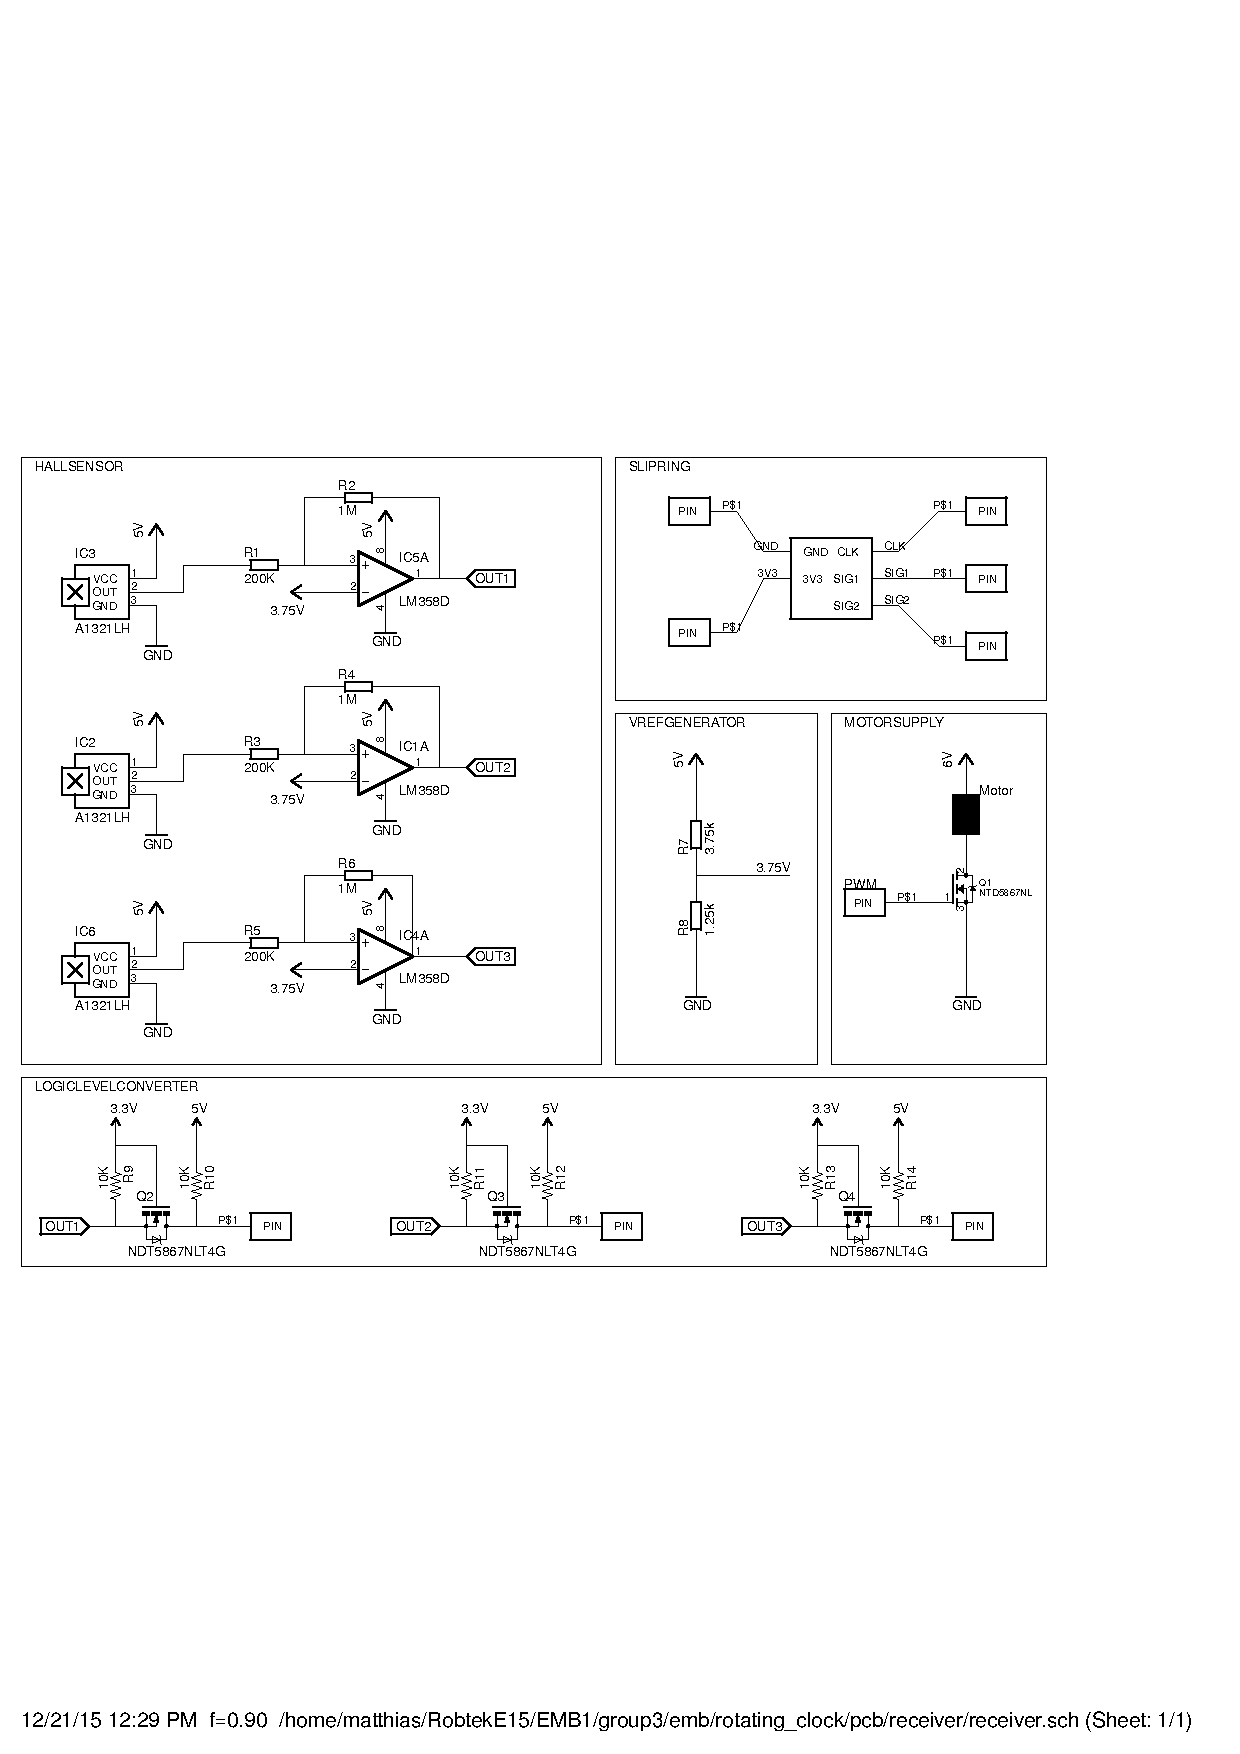
\includegraphics[scale=0.7,trim = 0 7cm 0 7cm,clip = true]{img/bottompcb_schematic}
 \caption{Schematic of the board that is mounted under the spinning board}
 \label{fig:botm_schematic}
\end{figure}

\subsubsection*{Resistor calculation for Schmitt trigger}
As mentioned in section \ref{sec:schmitt_cal}, the desired switching voltages for the Schmitt trigger are 4.5 and 3.5 V.
The resistor values R1-R6 are calculated using equation \ref{eq:calc_r1_r2}\cite{book:prac_ele}

\begin{equation}\label{eq:calc_r1_r2}
 \frac{R_1}{R_2} = \frac{\Delta V_{in}}{V_{cc}} = \frac{4.5V-3.5V}{5V} = 0.2V
\end{equation}
Chose 1 of the values, here $R_2$ = 1\ M$\Omega$
\begin{equation}
 R_1 = 0.2\cdot R_2 = 0.2\cdot 1 \text{M} \Omega = 200 \text{k}\Omega
\end{equation}

The reference voltage then has to be calculated in order to shift the hysteresis to the wanted values

\begin{equation}
 V_{ref} = \frac{V_{in1}}{1+\frac{R_1}{R_2}} = \frac{4.5V}{1V+0.2V} = 3.75 V
\end{equation}

\subsection{Slip Ring Connector}\label{sec:ring_connector}
The board with the LEDs will be rotating, making the communication to this board a problem.
Existing solutions called slip rings exist, but the ones in the price range of this project is rated for 250 rpm, which will be too slow for this project.
So a custom solution will be devised to combat this.

To make communication between the rotating board and the stationary FPGA, a slip ring connector is made.
This was made as two Eagle components so the sizes are identical.
In figure \ref{fig:slip_ring_eagle} is the slip ring shown.
The bottom layer contains rings where the signal is sent to.
The top layer has pads directly over the rings and by having a wire that touches the ring, the connection can be made.
The outer layers are used for signals.
This allows for multiple wires to have contact with the ring.
The power supply is stabilized with a $220 \mu F$ capacitor.
This is done to stabilize the power signal and to make sure the LED drivers does not disconnect if the wire loses contact for a moment.
The duration of this disconnect is hard to determine, so the a large capacitor is chosen to maximize the lifespan in case of a disconnect.

The LED driver requires a signal for power, ground, input signal, a clock and a latch.
Having multiple drivers does not increase the number of wires.

\begin{figure}[h]
 \centering
 \begin{subfigure}{0.4\linewidth}
 \centering
  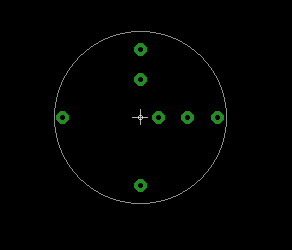
\includegraphics[width=0.8\linewidth]{img/slip_ring_top}
 \caption{Top layer.}
 \label{fig:slip_ring_top}
 \end{subfigure}
 \begin{subfigure}{0.4\linewidth}
 \centering
  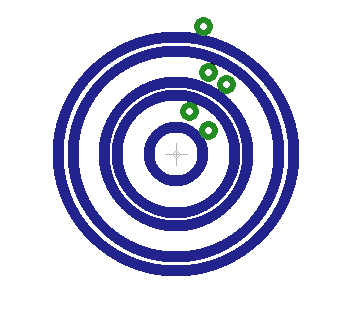
\includegraphics[width=0.8\linewidth]{img/slip_ring_bot}
 \caption{Bottom layer.}
 \label{fig:slip_ring_bot}
 \end{subfigure}
 \caption{Slip ring component made in Eagle.}
 \label{fig:slip_ring_eagle}
\end{figure}

\subsection{Top board}
On the top board all of the LEDs are placed, together with the most essential things needed in order to drive them.
The schematic can be seen in figure \ref{fig:top_board}
\begin{figure}
 \centering
 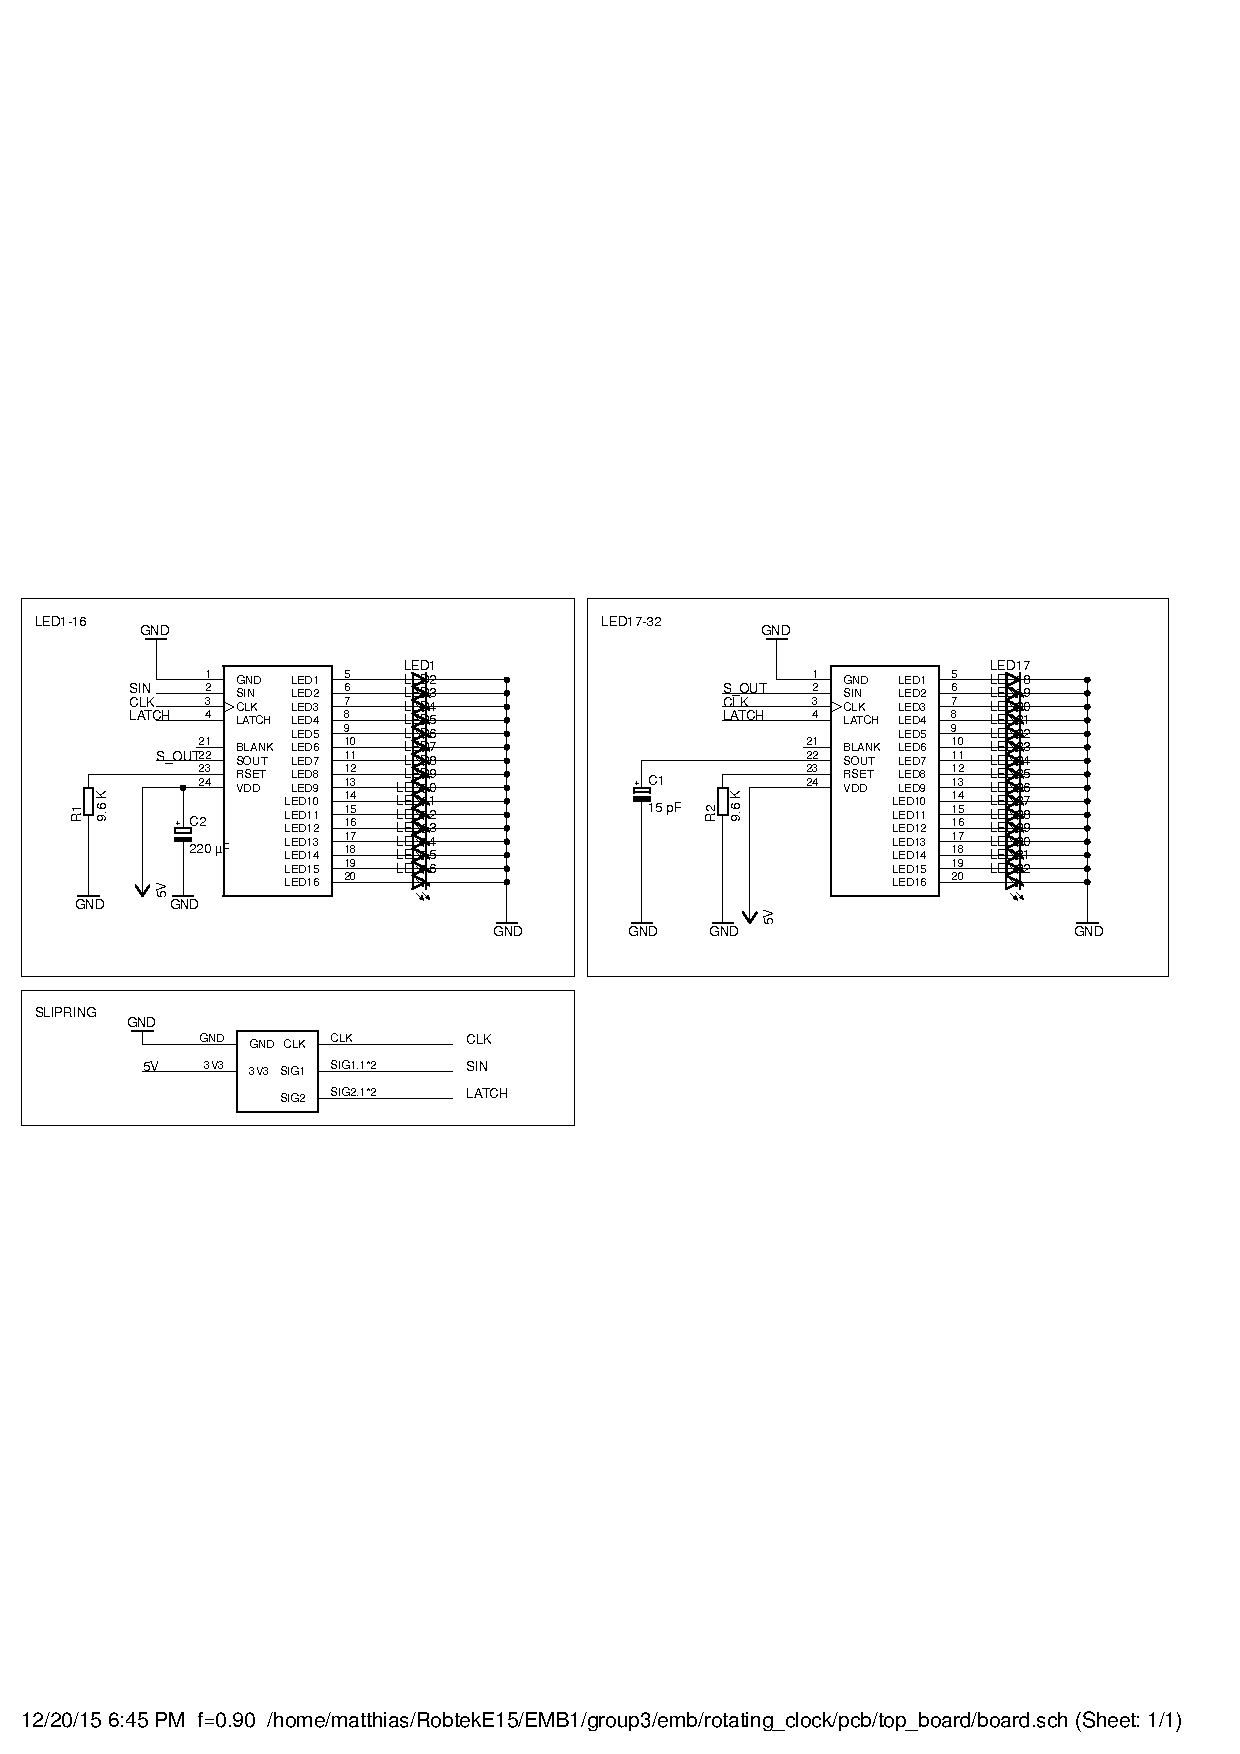
\includegraphics[width=\textwidth,trim=0 10cm 0 10cm,clip = true]{img/top_board}
 \caption{Schematic of the top board, made in Eagle CAD.}
 \label{fig:top_board}
\end{figure}

C2, the capacitor located on the VDD of the first LED driver is there in order to keep the LED drivers on even if there is a small period of time that the slip ring connector looses connection of VCC and GND.